% !TEX root = ../main.tex
%
\chapter{Vorgeschlagenes Wissensgraph\-konstruktions\-verfahren}%
\label{sec:text2kg}

Auf Basis der vorgestellten Konzeptgraphen, CoreNLP und PSL wird im folgenden Kapitel ein Verfahren für die online Konstruktion eines Wissensgraphen aus natürlichsprachlichen Textnachrichten aufgebaut.
Der Fokus liegt dabei primär auf der generellen Architektur des Verfahrens.
Das Resultat ist also als Proof-of-Concept zu verstehen, auf dessen Basis praxistaugliche Systeme konzipiert werden können.

\begin{figure}[h]
	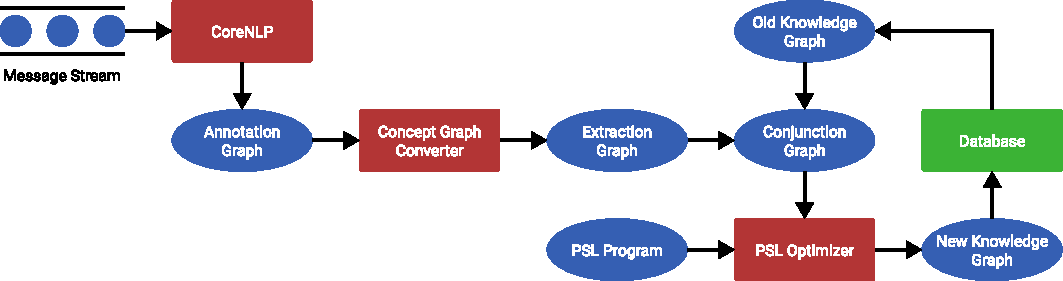
\includegraphics[width=\textwidth]{gfx/text2kg/architecture.pdf}
	\caption{Grobes Architekturdiagramm des Konstruktionsverfahrens}\label{fig:text2kg:architecture}
\end{figure}
Das im Folgenden vorgestellte Verfahren folgt einem dreistufigen Pipeline-Modell:
\begin{enumerate}
	\item Mittels CoreNLP wird eine eintreffende Textnachricht in einen Abhängigkeitsgraphen transformiert.
	\item Der resultierende Abhängigkeitsgraph wird in einen sog.\ Extraktionsgraphen umgewandelt.
		Hierbei handelt es sich um einen Konzeptgraphen, der den Inhalt der Nachricht formal repräsentiert.
	\item Der Extraktionsgraph wird mit dem bestehenden Wissensgraphen verschmolzen.
		Dies entspricht der Konjuktion der durch die beiden Graphen repräsentierten logischen Ausdrücke.
		Der resultierende Konjunktionsgraph wird als Eingabe für ein PSL-Programm verwendet, welches auf Basis des hinzugekommenen Wissens neue Beziehungen im Wissensgraphen inferiert.
\end{enumerate}
Die Beschreibung dieser Pipeline erfolgt in vier Abschnitten.
In \treft{sec:text2kg:implementation} wird kurz die technische Umsetzung erläutert.
\treft{sec:text2kg:ontology} beschreibt anschließend die Ontologie der konstruierten Wissensgraphen.
Nach diesen strukturellen Betrachtungen wird schließlich in \treft{sec:text2kg:nlp} und \treft{sec:text2kg:psl} die Transformation von Text zu Extraktionsgraph, bzw.\ von Extraktionsgraph zu Wissensgraph beschrieben.

\section{Implementation}%
\label{sec:text2kg:implementation}

\section{Wissensgraphontologie}%
\label{sec:text2kg:ontology}

\section{NLP-Phase}%
\label{sec:text2kg:nlp}

\section{Graphkonstruktionsphase}%
\label{sec:text2kg:psl}
